\documentclass[heading.tex]{subfiles} 
\begin{document}

\section{Introduction}

The hyperloop concept is a proposed transportation system aimed to lower costs and travel times relative to California's current high speed
 rail project. \cite{Musk} The design consists of a passenger pod traveling in a tube under light vacuum at ground level and near sonic
speeds. The capsule is supported by a set of air bearings with air provided by a battery powered compression system and propulsion maintained
by a set of linear actuators mounted to the tube. Even with the tube largely evacuated, the speed of the capsule is limited by the ability of air to
escape around the sides of the vehicle. This limitation is governed by the size of the capsule relative to the tube and is alleviated by redirecting air
through the inlet and compression system. Drawing sufficient airflow through the vehicle to support the bearings and achieve higher speeds results
in a fairly large air intake at the nose of the capsule, show in Fig. \ref{f:hyperloopCAD}. The diameter of this inlet and hence the diameter of the
capsule, is strongly tied to the maximum travel speed of the capsule. This coupling between the maximum velocity and
required tube diameter cascades into multiple subsystems and needs to be accounted for upfront in the design process. 
All of the sub-system interactions make it necessary to take a more integrated approach to the design of the Hyperloop concept. The intention of
this paper is to explore some of the most significant trade-offs between sub-systems and provide a starting point for subsystem expansion.

\begin{figure}[hbtp]
\centering
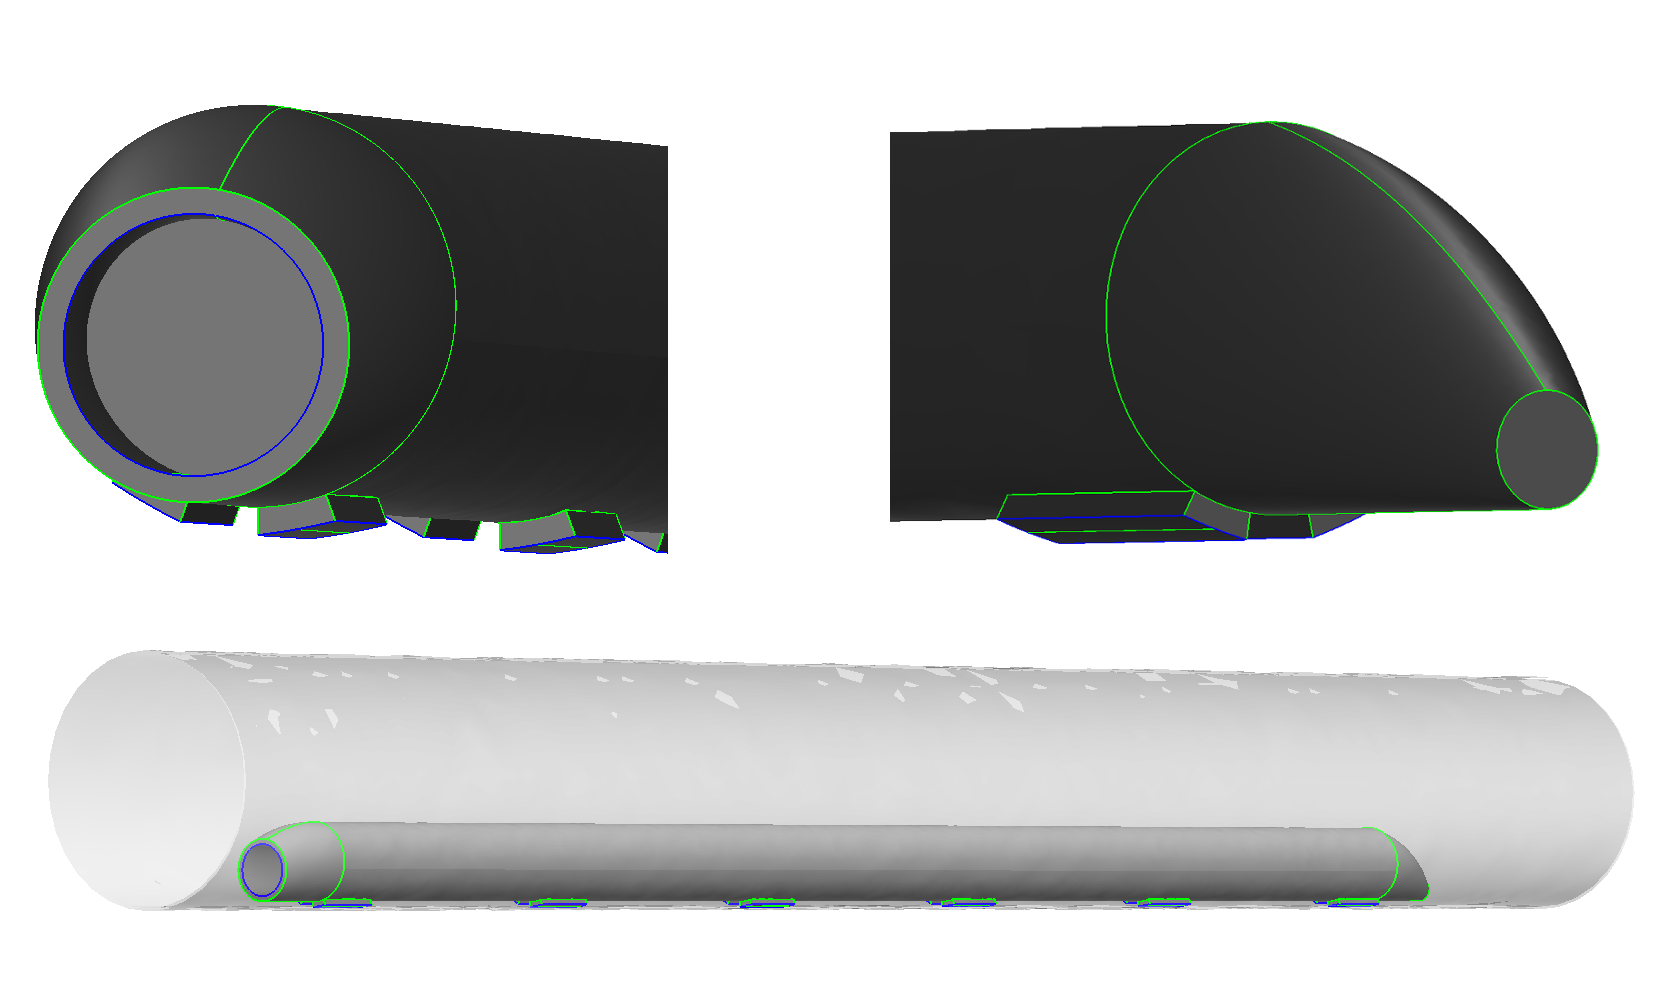
\includegraphics[scale=0.25]{images/hyperloop_cad.png}
\caption{Calculated baseline inlet (left), nozzle (right), and full assembly (bottom) for a capsule speed of Mach 0.8, rendered in OpenCSM a parametric solid modeler.}
\label{f:hyperloopCAD}
\end{figure}

The physical limitations of the system and the underlying design space needs to be better understood before ultimately approaching the
problem with the dual objectives of minimizing ticket cost and travel time. By identifying interactions and defining rigid interfaces between different
competencies the problem can
be kept tractable and development can be performed in parallel. The Hyperloop concept straddles a different combination of disciplines than many
existing monolithic systems, falling ambiguously between the purview of existing tool-sets and traditional engineering competencies. The modeling
approach described in this paper relies on the notion that the inlet, nozzle, and compression cycle within the passenger pod is not unlike those
found in aircraft concepts involving electric propulsion. They both operate at high speeds and low pressure conditions with an electric motor
driving turbo-machinery in a highly volume constrained vehicle. Therefore, experience drawn from systems design and optimization in aircraft engine
design were adapted for the capsule compressor analysis, heat estimates and capsule geometry. The full source code is provided in
 \cref{app:2} and external contribution is encouraged to expand, refine or replace models with higher fidelity analyses. The models solely rely on
free and easily accessible tool-sets with the Python programming language and OpenMDAO framework serving as the backbone for continued expansion.  

\subsection{Modeling Platform: OpenMDAO}
The presented Hyperloop models were built exclusively using open-source tools including, but not limited to: OpenCSM, GeoMACH, VSP and
Cantera. These models were subsequently connected and operated using the OpenMDAO framework. OpenMDAO is a Python based
integration environment that facilitates the application of advanced Multidisciplinary Design Analysis and Optimization (MDAO) methods.
The framework leverages the extensive scientific community already backing Python development and provides further tailored functionality
to more easily facilitate large and complex engineering problems. The development of this software is being led out NASA Glenn Research
Center with support from NASA Langley Research center, stemming from demands of unconventional aircraft concepts. Although NASA's
focus is centered on analyzing aerospace applications, the framework itself is extremely general and not specific to any discipline. As the
Hyperloop design evolves, an ever increasing number of design variables will need to be managed and optimized. OpenMDAO can provide
the means to manage this rapidly growing complexity in an efficient and flexible manner that will allow the model to grow as the necessary
refinements are made.

\section{Baseline Design}

Due to the novelty of the hyperloop design, the stack up of many subsystem uncertainties makes even the highest level trends difficult to pin down.
The initial subsystem modeling described below provides some concrete baseline numbers, since the devil is always in the implementation details. 

\subsection{Tube Diameter}
	The pod travels through a fixed diameter tube displacing air around itself. The tube air reaches the
pod with a relative velocity equal to the pod speed. As the air is forced through the smaller bypass area, it increases in speed. If you
assume a circular cross section for both the pod and tube, then the bypass air must travel through an area given by

\begin{equation*}
A_{bypass} = \pi(r_{tube}^2-r_{pod}^2)
\end{equation*}

Since $A_{tube}$ and the air density $\rho_{air}$ within the tube are both constant for given tube size, temperature and pressure, the mass flow rate of
the air traveling around the pod ($\dot{W}_{bypass}$) grows linearly with the velocity of the pod.

\begin{equation*}
\dot{W}_{bypass} = \rho_{air} A_{tube} V_{pod}
\end{equation*}

However, the velocity reaches a physical limitation as it reaches Mach 1. At this point, no additional flow can escape around the sides of the vehicle without
increasing the density of the air. For a given area ratio and flow conditions, the limiting pod speed can be determined.

\begin{equation*}
\frac{A_{tube}}{A_{bypass}} = \left(\frac{\gamma+1}{2}\right)^{-\frac{\gamma+1}{2\left(\gamma-1\right)}}\frac{\left(1+\frac{\gamma-1}{2}M^{2}\right)^{\frac{\gamma+1}{2\left(\gamma-1\right)}}}{M}
\end{equation*}


If the $V_{bypass}$ reaches the speed of sound, then the pod will act like a piston in a tube; increasing the air pressure in front
and lowering the pressure behind it. Without a ducted capsule the limiting speed is around 120 $\frac{m}{s}$, or Mach 0.3, as shown by the intersection of
the blue lines in figure \ref{f:flowLIMIT}. This limited pod speed is strongly dependent on the ratio of the pod diameter to the tube diameter.

\begin{figure}[hbtp]
\centering
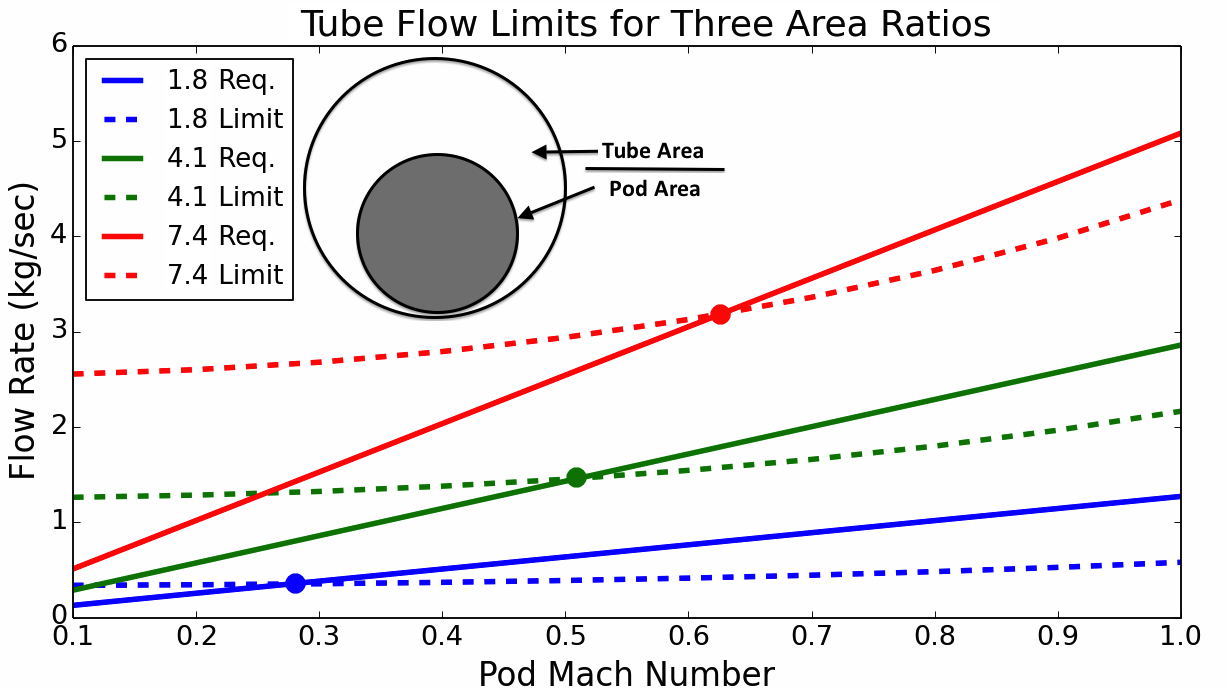
\includegraphics[width=\textwidth]{images/tube_flow_limit3.png}
\caption{Hyperloop speed limits as a function of three different area ratios}
\label{f:flowLIMIT}
\end{figure}

Such low speeds would not allow the hyperloop concept to significantly reduce travel times between Los Angeles and San Francisco relative to high speed rail.
To reach higher speeds, an inlet and compression system is needed to help push additional air through the pod. The amount
of air that the compression system needs to move is equal to the vertical distance between the required tube flow (the solid lines) and the choked flow limit
(the dashed lines) of figure \ref{f:flowLIMIT}. As speed increases, the flow demands on the compression system increases.

Additional non-linearity is introduced when considering the limitations of the compression system. Increasing the demands on the compression system
causes the required pod inlet diameter to grow in order to handle the increased flow. Traveling faster results in larger mass flow requirements, which drives
the pod diameter up, changing the area ratio and further increasing the mass flow requirements. This compounding relationship between 
speed and tube diameter is shown in figure \ref{f:machRAD}. The full system model converges on the minimal possible tube diameter, given a desired
pod Mach number with additional considerations for the steady state tube temperature and compressor performance.

\begin{figure}[hbtp]
\centering
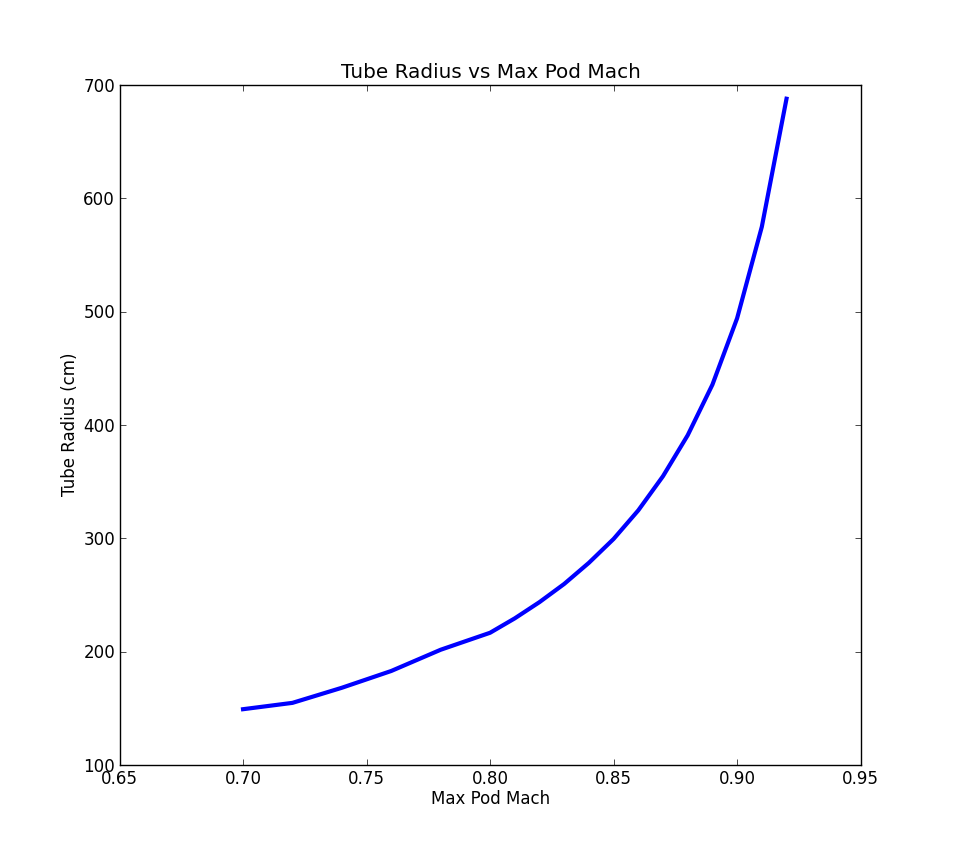
\includegraphics[scale=0.5]{images/mach_vs_rad.png}
\caption{Exponential relationship between pod speed and required tube radius}
\label{f:machRAD}
\end{figure}

Figure \ref{f:machRAD} portrays the exponential relationship between pod speed and required tube radius. This figure explicitly shows the trend depicted by
connecting the dots of figure \ref{f:flowLIMIT}. For visual simplicity (and as a more of a direct indicator of total system cost), the absolute tube radius is
charted rather than an area ratio. Although it isn't shown, the pod size is also varied at each optimized point. This plot assumes the capsule contains a
compression system and is therefore shifted further right than if the intersection points from figure \ref{f:flowLIMIT} were directly overlayed. 

The data shows that above Mach .85, the minimum allowable tube size gets very sensitive to pod travel speed. This indicates that speeds greater than Mach
.9 are likely not feasible. Even at a Mach .8, the tube diameter still needs to be around 4 meters, roughly
twice the size considered in the original proposal. With a maximum speed of Mach .8, the travel time is greater than 45 minutes. Additional time would also
be necessary to keep turns under 1 g. Although this performance is much less favorable than the performance
described in the original proposal, it still represents an improvement over what can be achieved with a high speed rail.

\subsection{Capsule Cooling Requirements}
The limits and requirements of a hypothetical on-board heat exchanger can be estimated with a straightforward energy balance. The
effectiveness of a heat exchanger can be described as the ratio of actual heat transfer over the maximum possible heat transfer. This can
be written mathematically as,

\begin{equation*}
{Q}_{released}  = effectiveness * {Q}_{max}
\end{equation*}


where Qmax=(Thot,in−Tcold,in)[m˙fluidCp,fluid]lowest with whichever fluid has the lowest product of m˙fluidCp,fluid

In order to satisfy the energy balance Qreleased=Qabsorbed , the following must be true,

\begin{equation*}
\dot{m}_{air} C_{p, air} (T_{out, air} - T_{in, air}) = {Q}_{released} = {Q}_{absorbed}= \dot{m}_{water} C_{p,water} (T_{out, water} - T_{in, water})
\end{equation*}

where the $T_{out}$  of each fluid is unknown. With assumed mass-flow rates and initial temperatures, a valid combination of Tout‘s of
each fluid can be found through solver iteration. Valid effectiveness levels for heat exchangers can be determined based on the E- NTU
method..

The effectiveness for a counter flow heat exchanger with a Cmin/Cmax of ~0.25 was chosen 

The following conditions satisfied an energy balance with an assumed effectiveness of 0.9765, and the proposed requirement to cool the
air completely down to inlet temperatures.

\begin{tabular}{|c|c|c|c|c|c|c|}
\hline 
Fluid & Cp & Tin & Tout & mdot & Q (kJ/s) & Qmax \\ 
\hline 
Air & 1.006 kJ/kh-K & 791 K & 300 K & 0.49 kg/s & -242 & 247.9 \\ 
\hline 
Water & 4.186 kJ/kg-K & 288.15 & 416.6 K  & 0.45 kg/s & 242 & 247.9 \\ 
\hline 
\end{tabular} 

With a 35 minute trip, 0.45kg/s∗60s/min∗35min=945kg of standard temperature/pressure water would need to be carried with appropriate
sized steam tanks. This doesn't even account for the second stage heat exchanger, making the system nearly infeasible with water and
unpressurized tanks. Various systems involving alternate coolants such as liquid air or pressurized tanks could be explored.

Further discussion of heat exchanger sizing and tube equilibrium temperature can be found in the Tube Temperature section of the
‘Subsystem Modeling Theory’ chapter of the docs.

\subsection{Sensitivity}
\begin{figure}[hbtp]
\centering
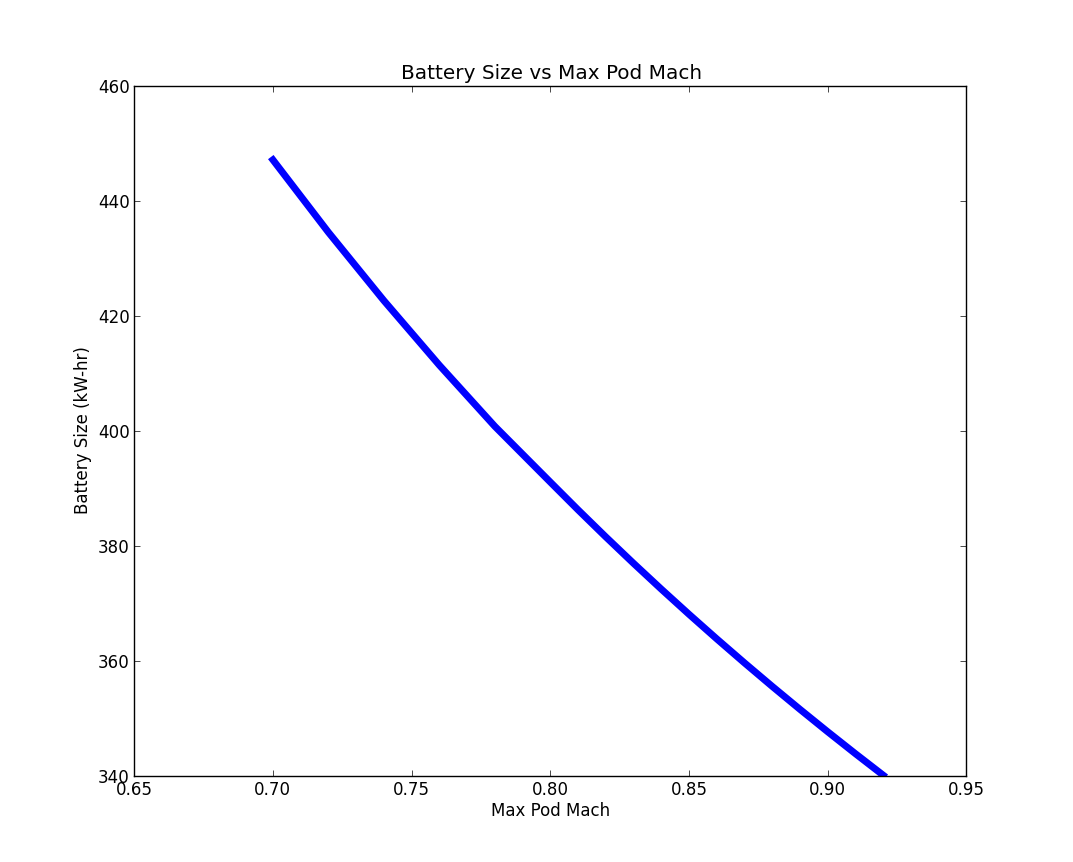
\includegraphics[scale=0.5]{images/mach_vs_energy.png}
\caption{Hyperloop speed limits as a function of tube radius}
\end{figure}

\section{Subsystem Modeling Theory}

The following sections some of the engineering behind the models. Our main focus was to produce a model that predicts the instantaneous
power required to run a transport capsule at the conditions specified in the original work. These power requirements are a function of the
capsule air cycle and thermal conditions. The resultant power could then be combined with the estimated travel time to size the battery
and coolant storage requirements. The following section provides a brief summary of the assumptions and modeling that went into each
sub-system necessary to perform this analysis.

For the sake of conciseness, each section serves as a general summary. The reader is recommended to refer to the actual source code and
included documentation for full implementation details. The current model omits economic, structural, safety, and infrastructure
considerations; areas that become more prominent once the core engineering concept is deemed sufficiently feasible. These aspects are
equally important to the overall design and they represent the next required step in producing a viable hyperloop design concept.

\subsection{Compression System}

The compression system performs two functions on the hyperloop concept.
Pressurizes some of the air, increasing its density, to provide a means of exceeding the Kantrowitz limit.
Provides a source of high pressure air to the air bearing system.
Each of these functions requires that the compressors move a certain amount of air, which combine to define the total airflow for the whole
sub-system. The system is comprised of an inlet, two compressors, two heat exchangers, a nozzle, and a duct to air bearings.

\begin{figure}[hbtp]
\centering
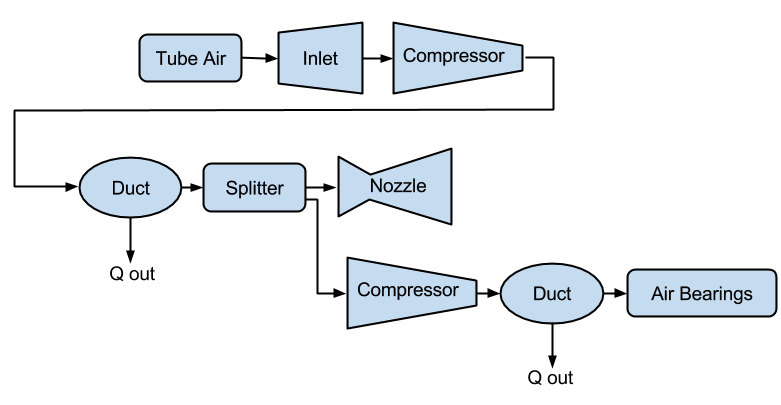
\includegraphics[scale=0.5]{images/compressor_schematic.png}
\caption{Schematic flow diagram of the compressor system}
\end{figure}

The compression systems is modeled as a 1-D cycle, representing components as a thermodynamic processes which are chained together.
These models predict the instantaneous power consumption of the compression system.

\subsection{Tube Temperature}

As each pod passes through the tube, it adds energy to the air in an amount equivalent to what was used to power the compressors. This
added energy will cause a small temperature rise in the tube. Each pod causes an additional slight temperature rise as it passes, which could
potentially heat the overall hyperloop system to excessive temperatures. In the original proposal, to combat this effect, it was proposed
that water-to-air heat exchangers could be added to the compression system. These would use water stored in tanks in the pod to cool the
air by converting it to steam. The steam could then be stored in an additional tank, and offloaded once the pod reached its destination.
According to our initial calculations, using water for cooling is not an ideal design for two reasons:

1) The flow rate of water needed to remove the heat added by the compressors is very large, and storing the resulting steam would result
in an unreasonably large pod (over 200 meters long).

2) The heat addition from each pod compressor cycle is fairly low relative to other heat transfer mechanisms, such as radiative solar
heating of an uncovered steel tube. Even without an active on-board cooling solution, the tube temperatures may not reach excessive
levels.

In the following two sections, we explain the analyses we used to draw the above conclusions.

\subsubsection{Heat Exchanger Design}

In spite of the results in the capsule cooling section, on-board cooling could possibly be used to partially fulfill cooling requirements. As a
basic exercise a hypothetical baseline heat exchanger model was developed to investigate the weight and sizing requirements of an 
on-board water cooling system using the Logarithmic Mean Temperature Difference (LMTD) method. \cite{Cengal} \cite{Turns} The
exchanger was sized to remove all excess heat generated by the two compressors using a pedagogical shell and tube design. Based on the
temperature restraints and exhaust flow rate determined by the cycle model, necessary water flow rates were calculated to ensure an
energy balance. Given a predefined heat exchanger cross-section, fluid flow regimes and heat transfer coefficients were obtained. The
combination of all of these elements provide a first-cut approximation of tank sizes, total heat exchanger volume, and pumping
requirements.

Given:

-For simplicity, only a single heat exchanger is designed (to cool down the air coming off the first compressor stage)

-Sized as a classic shell and tube heat exchanger

-Input and output temperatures are known for each fluid

-Temperature change across the heat exchanger cannot be so large that Cp changes significantly

-Rigorously defined for double-pipe(or tubular) heat exchanger

With a chosen cross-sectional area of pipe and annulus, and known Q and mdot, the velocity of each fluid can be determined.

\begin{equation*}
\dot{m} = \rho A V     ...therfore...        V  = \frac{Q} {\rho A C_{p} (T_{out} - T_{in})}
\end{equation*}
The hydraulic diameter (characteristic length) of a tube can also be calculated as,
\begin{equation*}
D_{h} = \frac{4 A_{f}} {P_{f}}  = \frac{4 \pi (ID_{a}^2-OD_{p}^2)} {4 \pi (ID_{a}+OD_{p})} = ID_{a}-OD_{p}
\end{equation*}
\begin{equation*}
D_{\varepsilon} = \frac{4 A_{f}} {P_{ht}}   =  \frac{4 \pi (ID_{a}^2-OD_{p}^2)} {4 \pi (ID_{a}*OD_{p})} = \frac{ID_{a}^2-OD_{p}^2}{OD_{p}}
\end{equation*}
Based on the geometry, kinematic viscosity  $\upsilon$ , dynamic viscosity  $\mu$ , thermal conductivity k, and velocity of the fluids the
following non-dimension values can be calculated

Reynolds Number: (inertial forces/ viscous forces)  Re = $\frac{V D_{h}} {\upsilon}$

Prandtl Number: (viscous diffusion rate/ thermal diffusion rate)  Pr = $\frac{C_{p} \mu} {k}$

Based on the flow regimes determined above, the Nusselt Number.. can be calculated. The Dittus-Boelter equation is used in this case,

Nusselt Number: (convective heat transfer / conductive heat transfer)  Nu = $0.023*(Re^{4/5})*(Pr^{n})$ where n = 0.4 if the fluid is heated, n = 0.3 if the fluid is cooled.

Subsequently the convective heat transfer coefficient of each fluid can be determined,  h = $\frac{Nu*k} {D_{\varepsilon}}$

All of these terms can then be used to calculate the overall heat transfer coefficient of the system,

\begin{equation*}
U_{o} = \frac{1} {(\frac{A_{o}}{A_{i}h{i}}) + (\frac{A_{o}ln(\frac{r_{o}}{r_{i}})}{2 \pi k L}) + \frac{1}{h_{o}}}
\end{equation*}
\begin{equation*}
\Delta {T}_{LMTD} = \frac{\Delta {T}_{2}-\Delta {T}_{1}}{ln(\frac{\Delta {T}_{2}}{\Delta {T}_{1}})}
\end{equation*}
\begin{equation*}
\Delta {T}_{1} = T_{hot,in} - T_{cold,out}
\end{equation*}
\begin{equation*}
\Delta {T}_{2} = T_{hot,out} - T_{cold,in}
\end{equation*}
allows the length to be determined for a single pass heat exchanger.
\begin{equation*}
q = U_{o} \pi D_{o} L \Delta {T}_{LMTD}
\end{equation*}
Further calculations for the multipass heat exchanger can be found in the source code.


\subsubsection{Equilibrium Tube Temperature}
A high-level assessment of the overall steady-state heat transfer between the 300 mile hyperloop tube and the ambient atmosphere was
also investigated. The outer diameter of the pipe was chosen as the control surface boundary. Heat added from the capsule exhaust air and
solar flux were considered the primary drivers for heat absorption into the tube. Heat released from the tube was modeled by means of
ambient natural convection, and radiation out from the stainless-steel surface. The thermal interaction between the rarified internal air and
tube was not modeled and assumed to reach steady-state in a reasonable period of time. These calculations served to approximate the
necessary cooling requirements of the on-board heat exchanger given a certain steady-state heat limit within the tube.

The heat being added by the pods can be determined from the cycle analysis, or based purely on inlet total temperatures with isentropic
flow relations.

\begin{equation*}
T_{t} = T_{s} * [1 + \frac{\gamma -1}{2} MN^2]
\end{equation*}
\begin{equation*}
P_{t} = P_{s} * (\frac{ T_{t}}{T_{s}})^(\frac{\gamma}{\gamma -1})
\end{equation*}
\begin{equation*}
P_{t,exit} = P_{t,inlet} * PR
\end{equation*}
\begin{equation*}
T_{t,exit} = T_{t,inlet} + \frac{([T_{t,inlet}*PR^{(\frac{\gamma-1}{\gamma})}] - T_{t,inlet})}  {{\eta}_{adiabatic}}
\end{equation*}

Where PR is the compressor pressure ratio, MN is the mach number,  $\gamma$ is the specific heat ratio, and  ${\eta}_{adiabatic}$ is the
adiabatic efficiency.

With the air flow rate known, the heat flow rate per capsule is obtained,

\begin{equation*}
{Q}_{pod}= \dot{m}_{air} C_{p,air} (T_{out, air} - T_{tube})
\end{equation*}
The peak heating rate from the pods scales linearly.
\begin{equation*}
{Q}_{peak}= Q_{pod} (\# ofpods)
\end{equation*}
The solar heat flow per unit area can be approximated, given the solar reflectance index (SRI) of stainless steel, non-normal incidence factor
of the cylinder and solar insulation (SIF).
\begin{equation*}
Solar = (1-SRI) {\theta}_{nni} SIF
\end{equation*}
Multiplying this by the viewing area of the tube (assuming no shade and constant sun)
\begin{equation*}
Q_{solar} = Solar * A_{view} = Solar * L_{tube} * OD_{tube}
\end{equation*}
Tube cooling can be attributed to two general mechanisms, radiation and natural convection. Radiation power per unit area can be
approximated to
\begin{equation*}
\frac{P_{rad}}{A} = \epsilon \sigma (T_{pipe}^4 - T_{ambient}^4)
\end{equation*}
where  $\epsilon$ is the emissivity factor and  $\sigma$ is the Stefan-Boltzmann constant.

Multiplying by the surface area of the tube, the total heating rate can be found,
\begin{equation*}
P_{rad} =  \frac{P_{rad}}{A} * \pi L_{tube} OD_{tube}
\end{equation*}

Assuming the worst case scenario of no cross wind, convection is primarily driven by temperature gradients. The non-dimensional relation
between buoyancy and viscosity driven flows is parameterized using the following empirical constants. \cite{Berton} \cite{Incropera}

if 150 K <  $T_{amb}$ < 400 K:

\begin{equation*}
\frac{g \beta T} {\upsilon^2} = (m^{-3}K^{-1}) = 4.178\times10^{19} \times T_{amb}^{-4.639}
\end{equation*}

\begin{equation*}
Pr = 1.23 T_{amb}^{-0.09685}
\end{equation*}

if 400 K <  $T_{amb}$ < 2100 K:


\begin{equation*}
\frac{g \beta T} {\upsilon^2}  = (m^{-3}K^{-1}) = 4.985\times10^{18} \times T_{amb}^{-4.284}
\end{equation*}
\begin{equation*}
Pr = 0.59 T_{amb}^{0.0239}
\end{equation*}
The Grashof Number can then be approximated,


\begin{equation*}
Gr = \frac{g \beta T} {\upsilon^2}  (T_{tube}-T_{amb}) {OuterDiameter}_{tube}^3
\end{equation*}
The non-dimensional Rayleigh number can then be calculated to estimate buoyancy effects, leading to the Nusselt number.


\begin{equation*}
Ra = Gr * Pr
\end{equation*}
\begin{equation*}
Nu = \Bigg(0.6 + \frac{0.387Ra^{\frac{1}{6}}}{[1+(\frac{0.559}{Pr})^{\frac{9}{16}}]^{\frac{8}{27}}}\Bigg)^2
\end{equation*}

From this point the total heat transfer from natural convection can be obtained,

\begin{equation*}
Q_{nat. conv} = hA \Delta T = \frac{k*Nu}{ {OD}_{tube}} \pi {L}_{tube} {OD}_{tube} (T_{tube}-T_{amb})
\end{equation*}

The steady state tube temperature can be found by varying the tube temperature until the rate of heat being released from the tube
matches the rate of heat being absorbed by the tube. Using the values provided in the source code, a steady state temperature of 120 F
was reached.


\section{Model Layout}
The model is broken down into 5 major assemblies as described below. 

\begin{enumerate}
  \item Compression System (\texttt{compress}): Performance and power consumption of the compressors
  \item Mission Analysis (\texttt{mission}): Estimate of travel time
  \item Pod Geometry (\texttt{pod}): Physical dimensions of the capsule and calculations that depend on them
  \item Tube Flow Limitations (\texttt{flow\_limit}): Pod speed limitations based on choked flow restrictions between the pod and the tube
  \item Tube Wall Temperature (\texttt{tube\_wall\_temp}): Equilibrium temperature of the tube wall
\end{enumerate}

The connectivity between the assemblies is visually represented using XDSM charts below. Each green box represents a system that takes a
set of inputs and operates on them to produce a set of outputs. The connection of one system's outputs to another system's inputs is
visualized as a grey line. The cascading parallelograms indicate intersections, implying that an output is connected to multiple inputs. 


\begin{figure}[hbtp]
\centering
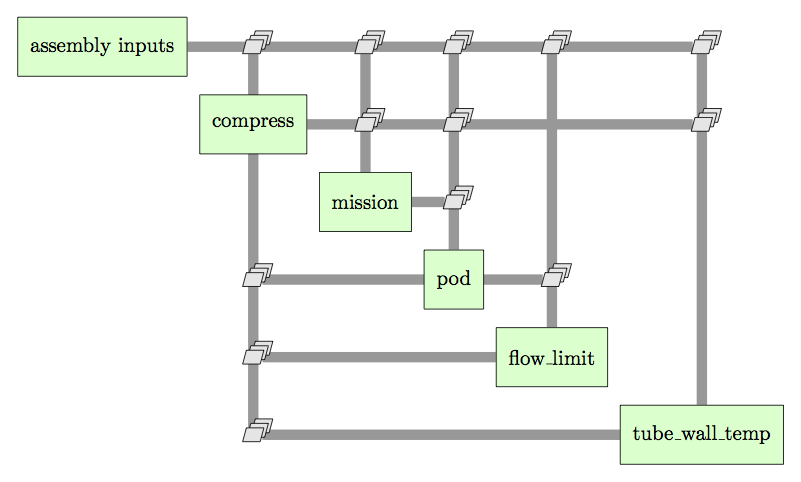
\includegraphics[scale=1]{images/hyperloop_assembly_xdsm.png}
\caption{Hyperloop Top Level Assembly XDSM}
\label{f:hyperloopXDSM}
\end{figure}

The compression system and pod geometry systems in figure \ref{f:hyperloopXDSM} are further expanded into sub-assemblies as shown in figure \ref{f:podXDSM} and \ref{f:compressorXDSM}.

\begin{figure}[hbtp]
\centering
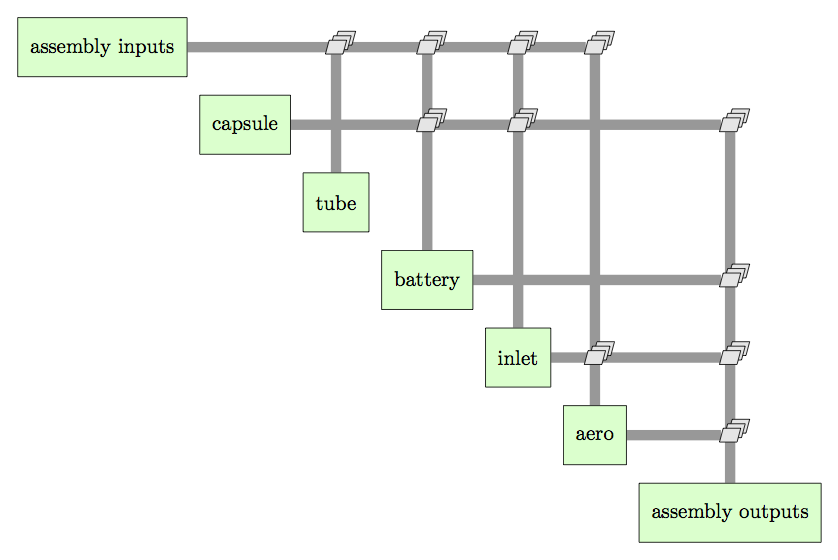
\includegraphics[scale=1]{images/pod_assembly_xdsm.png}
\caption{Expanded \texttt{pod} assembly XDSM}
\label{f:podXDSM}
\end{figure}

\begin{figure}[hbtp]
\centering
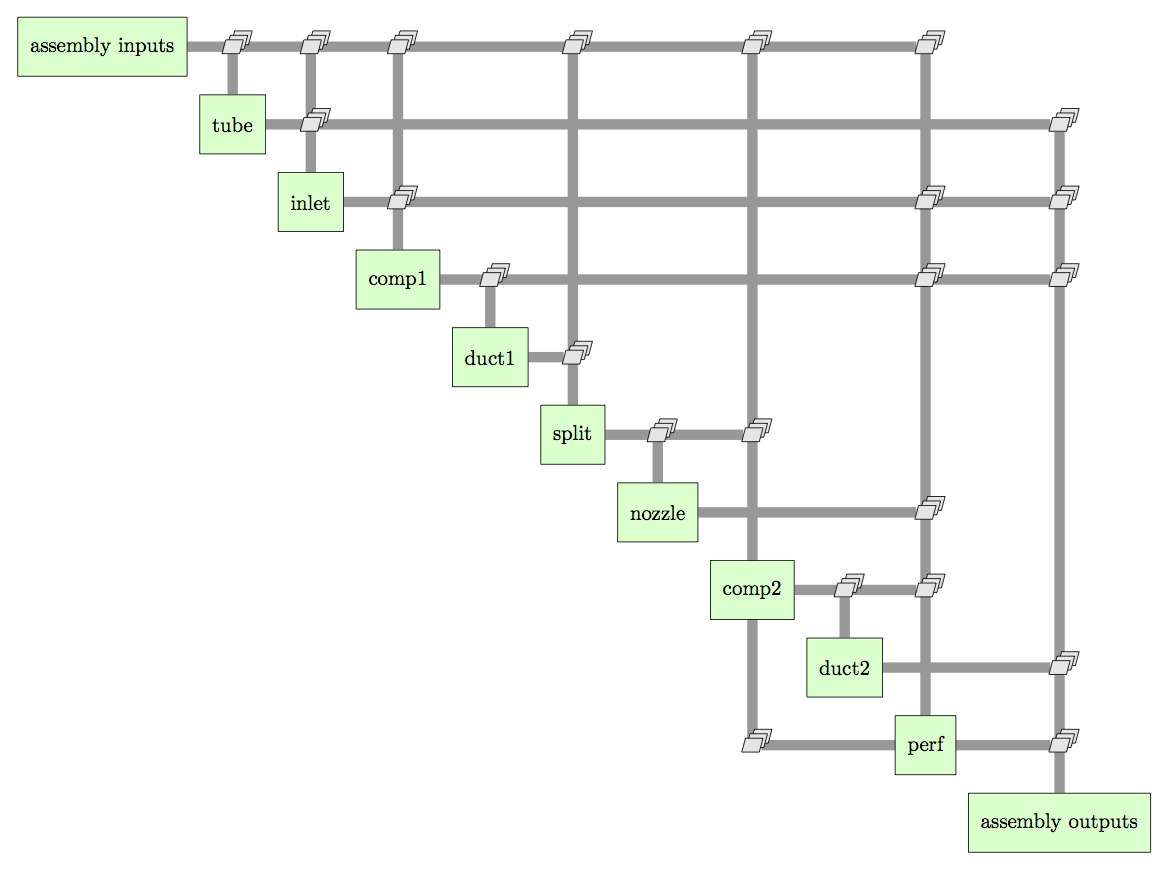
\includegraphics[scale=0.75]{images/compress_assembly_xdsm.png}
\caption{Expanded \texttt{compress} assembly XDSM}
\label{f:compressorXDSM}
\end{figure}

\subsection{Design Variables}
The system design is defined at the top-most level with the following design variables. These variables can be actively varied
 by the optimizer to achieve user defined objectives:

\begin{adjustwidth}{-3cm}{-3cm}
\begin{tabular}{|c|c|c|c|c|c|}
\hline 
Variable & Description & Units & Baseline Val. & Min & Max \\ 
\hline 
\texttt{Mach\_bypass} & Mach number of the air traveling around the pod & - & 0.95 & 0.5 & 0.98 \\ 
\hline 
\texttt{Mach\_pod\_max} & Maximum travel Mach number of the pod & - & 0.9 & 0.5 & 0.98 \\ 
\hline 
\texttt{Mach\_c1\_in} & Mach number of the air at the back of the inlet & - & 0.6 & 0.5 & 0.8 \\ 
\hline 
\texttt{Ps\_tube} & Static pressure of the air in the tube & Pa & 99 & 99 & 500 \\ 
\hline 
\texttt{c1\_PR\_des} & First compressor pressure ratio & - & 12.47 & 10 & 25 \\ 
\hline 
\end{tabular} 
\end{adjustwidth}

\subsection{Model Parameters}
These variables are free for the user to set, but are not intended for the optimizer. Rather, they are general traits of the system.

\begin{adjustwidth}{-3cm}{-3cm}
\begin{tabular}{|c|c|c|c|c|c|}
\hline 
Variable & Description & Units & Baseline Val & Min. & Max. \\ 
\hline 
pwr\_marg & Safety factor applied to the power requirement for the pod & - & 0.3 & 0 & 2 \\ 
\hline 
solar\_heating\_factor & Fraction of solar radiation to consider in tube temperature & - & 0.7 & 0 & 1 \\ 
\hline 
tube\_length & Length of the tube & m & 563270 & - & - \\ 
\hline 
n\_rows & Number of rows of seats in the passenger capsule & - & 14 & - & - \\ 
\hline 
length\_row & Length allotted to each row of seats & cm & 150 & 120 & 200 \\ 
\hline 
coef\_drag & Drag Coefficient for the pod & - & 2 & 0.6 & 2.5 \\ 
\hline 
hub\_to\_tip & Ratio of hub radius to tip radius for the first compressor & - & 0.4 & 0.2 & 0.6 \\ 
\hline 
\end{tabular} 
\end{adjustwidth}

\subsection{Constraints and State Variables}

The hyperloop concept presents a multidisciplinary design problem and encapsulating complexity into systems makes the relationship
between variables easier to understand.  Any connection originating from the left side of a component in an XDSM diagram represents a
cyclic connection. The cyclic connections in figure \ref{f:hyperloopXDSM}  and \ref{f:compressorXDSM} represent the coupling relationships
between the sub-systems. These couplings enforce a set of equality constraints that must be satisfied for any physically valid hyperloop design. 

\begin{equation} \label{eq:flow}
	0.01*(\texttt{compress.W\_in} - \texttt{flow\_limit.W\_excess}) = 0
\end{equation}
\begin{equation}
	\texttt{compress.Ps\_bearing\_residual} = 0
\end{equation}
\begin{equation}
	\texttt{tube\_wall\_temp.ss\_temp\_residual} = 0
\end{equation}
\begin{equation} \label{eq:area}
	0.01*(\texttt{pod.area\_compressor\_bypass} - \texttt{compress.area\_c1\_out}) = 0
\end{equation}

For constraints \ref{eq:flow} and \ref{eq:area}, a multiplier has been applied to the constraint to scale it for improved numerical
convergence.

The optimizer varies  the following state variables to to satisfy the constraints. 

\begin{enumerate}
\item \texttt{compress.W\_in}
\item \texttt{compress.c2\_PR\_des}
\item (\texttt{compress.Ts\_tube}, \texttt{flow\_limit.Ts\_tube}, \texttt{tube\_wall\_temp.temp\_boundary}) \label{Temp}
\item (\texttt{flow\_limit.radius\_tube}, \texttt{pod.radius\_tube\_inner}) \label{Radius}
\end{enumerate}

State variables \ref{Temp} and \ref{Radius} are given as a list of variables signifying that they are linked variables with equivalent values. They are
treated as a single variable for the purposes of converging the model, but remain as distinct variables within each subsystem.

\subsection{Outputs}
There are a number of output values that are of interest

\begin{description}
  \item[Overall pod radius] \hfill \\
  \texttt{pod.radius\_inlet\_outer}
  \item[Total mass flow through the compression system] \hfill \\
  \texttt{compress.W\_in}
  \item[Total power required to drive the compression system] \hfill \\
  \texttt{compress.pwr\_req}
  \item[Total energy needed to power the compression system for one trip] \hfill \\
  \texttt{mission.energy}
  \item[Travel time for one trip] \hfill \\
  \texttt{mission.time}
  \item[Maximum speed] \hfill \\
  \texttt{compress.speed\_max}
  \item[Equilibrium tube temperature] \hfill \\
  \texttt{tube\_wall\_temp.temp}
\end{description}

Note: For a more complete design process, the values of the design variables would be optimized to minimize a combination of total power
consumption and travel time. However, the model does not currently calculate some key values needed to get a useful answer. In particular,
the linear accelerator and vacuum pump power needs to be modeled before a design optimization can be attempted.
It should be noted that you can select designs that are not realistic, particularly with respect to \texttt{pod.radius\_inlet\_outer}. There is
a strong relationship between \texttt{Mach\_pod\_max} and the \texttt{pod.radius\_inlet\_outer}. If you select a high 
\texttt{Mach\_pod\_max} (Above .8), you may find that the radius has shrunk below what is physically feasible without significant design
changes.

\section{Future Modeling Road Map}
The current model of the hyperloop focuses on some of the primary sub-systems that operate within the pod. However, there is much more
analysis that needs to be done to build a complete hyperloop model. Below provides a brief summary of the areas we feel represent the
logical next steps for the engineering aspects of the analysis.

\subsection{System Design Optimization}
The current baseline appears to be a feasible design, but the design space is large (and will grow with additional models) and needs to be
more fully explored. Overall, the goal of the hyperloop design should be to find the right compromise between maximum passenger
throughput, minimum travel time, and minimum cost per trip. The following are some major open questions about the hyperloop design
space:

1) What is the relationship between overall energy usage and tube pressure? Would a slightly higher pressure lower the overall energy
consumption by reducing vacuum pump effort more than it increases power requirements for the pod?

2) What is the best combination of pressure ratios for the compression system? Does the bypass air need to be pressurized so highly?

3) What is the best size for the tube diameter? Larger diameters will increase pump effort, but decrease pod power usage? Could a larger
diameter coupled with a slightly higher pressure provide superior performance?

\subsection{Geometry}
This model makes some simple geometric calculations, however a real parametric geometry model needs to be included. This model is
necessary to properly consider the layout and packaging issues involved in the design, but it also needed to do more complete structural
analyses on the pressurized containers as well as to do an aerodynamic shape optimization of the outer shape.

Some alternate configurations could possibly considered as well. Although the length of the capsule would grow by a factor of almost 2, it
might be possible to put the seats in a single file layout to reduce the overall tube dimensions. The effect of this change on the overall
system is not obvious and needs to be studied.

The geometry model needs to be built in an open source geometry system so that it can be freely shared with the rest of the model.

\subsection{Battery and Motors}
The initial estimates of battery size and weight rely on ridiculously simple calculations. As noted, the power requirements amount to roughly
3 to 5 battery packs from a Tesla Model-S. Much better weight and size estimates for these off-the-shelf batteries need to be integrated.

No work has been done to size the motors or account for any cooling requirements they might need. Although the current results indicate
that a cooling system for the compressed air is not needed, you may still need something to cool the batteries and motors. The power
requirements, weight, and space needs of such cooling systems needs to be considered.

\subsection{Air Bearings}
The current models assume a fixed mass flow requirement for the air bearing system. A more accurate model would account for the overall
weight of the pod, the pressure of the air, and the overall bearing size. A more detailed bearing model should be coupled to the
compression system model to ensure a feasible design is achieved.

In addition, some investigations need to be made into the lower speed operation of the pod. It's possible that splitting the compression
system into two independent paths would be beneficial, if the bearings require a relatively constant mass flow rate and pressure, because it
would allow a more flexible operation of what is currently the first stage compressor.



\subsection{Vacuum Pumps}
The current model indicates that a tube with around a 4 meter diameter will be needed to reach the high velocities to keep the travel time
to around 35 minutes. The size of the tubes will impact to key power requirements for the vacuum pumps:

The peak power requirements to pump the tubes down in a reasonable time
The steady state power requirements to maintain the high vacuum in the tube
Both of these aspects need to be modeled and incorporated into the system models.


\subsection{Solar Power Generation}
One of the proposed features of the hyperloop concept is its near net-zero energy consumption, via the inclusion of solar panels along the
length of the tubes. Models are needed to predict, based on geographical location, weather, and time of year, how much power could be
produced on an ongoing basis from such a solar panel system.

The power production and power consumption of the hyperloop system need to be compared. Even assuming you can reach a net zero
energy usage on an average basis, the timing of the production and consumption has a strong impact on how much energy storage is
necessary in the overall system. This will have an impact on it's overall cost.

\subsection{Pod Structural Design}
The passenger pod is, from a structural perspective, a pressure vessel experiencing a fairly pressure ratio of around 1000. The original
design concept calls for a non-circular pressure vessel which raises some structural design issues. It's possible to design an effective
structure using modern aircraft grade composites technologies, but it's possible that a round cross section could allow for a more
traditional construction and reduce costs. Structural models considering composites and metallic construction are needed.

\subsection{Component Mass Estimation}
The current model does not include any significant weight estimation. Every part of the model needs to have weight estimates added.

\subsection{Linear Accelerators}
These are not considered at all currently. However, they will obviously need to be modeled as part of the mission analysis work.

\subsection{Route Optimization}
The current mission analysis takes the velocity profile in the original proposal as a given. We normalize this profile in both time and velocity,
then integrate it. This gives a speed factor of about .8. So for any given maximum velocity, the average velocity would be about 80% of it.

While this simple method provides some basic dependence of travel time on overall speed and tube length it is not really sufficient. A more
advanced analysis needs to be constructed which accounts for actual passenger G-load constraints and can derive an optimal route and
speed profile for a given design.

\begin{figure}[hbtp]
\caption{Velocity profile given in the original proposal}
\centering
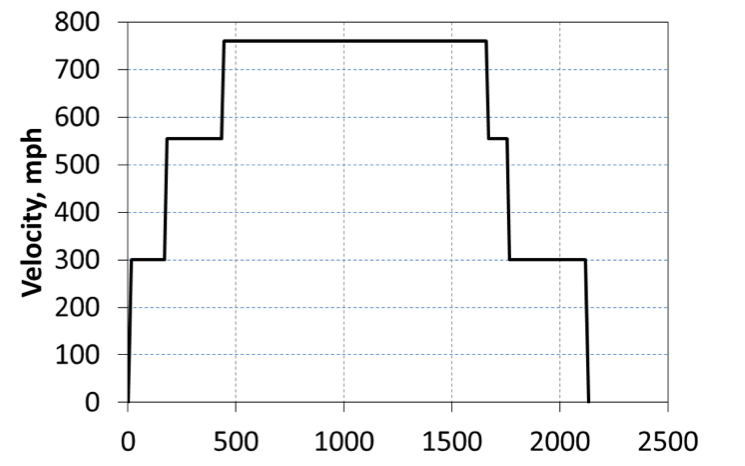
\includegraphics[scale=0.5]{images/velocity_profile.png}
\end{figure}

\section{Contributing}
This plugin is designed to be a jumping off point for community contributions to help crowd source the development of the hyperloop
concept. The readme on the github repository walks through basic installation steps, further support can be found through the main
OpenMDAO docs. And the basic structure of an assembly is explained in the usage section of these docs.

\section{Conclusions}
For the most part, the ideas and numbers given in the original hyperloop proposal hold up using this analysis. However, the data shows that
there are two major changes to the design that need to be considered.

The tube cross section will need to be significantly larger than the original proposal. In the original proposal, the tube was sized with a diameter 2.23
meters. However, it appears that it will need to have a diameter closer to 4 meters to reach speeds maximum speeds of Mach 0.8.
On-board water based inter-coolers also seem impractical due to both volume and weight constraints. This may prove to be a non-issue since
temperature rise due to compression is significant less than originally estimated and only leads to a modest rise in steady-state tube
temperature. Assuming the tube was left uncovered, the heat rate from solar radiation would be an order of magnitude larger than the heat
rate added from pod compression systems. Further assuming a 90 degF day, radiation and convection out of the tube would lead to a
manageable steady state tube wall temperature of 120 degF.

%\begin{thebibliography}{WoodTP}
%\bibitem[WoodTP]{woodTP} Wood, W.A., ``Multidimensional Upwind
 % Fluctuation Splitting Scheme with Mesh Adaption for Hypersonic Viscous
 % Flow,'' NASA/TP 2002-211640, Apr.~2002.
%\end{thebibliography}
%{\em Note that this entry is not necessarily in the correct NASA
%  format. Consult Technical Editing for correct reference format.}
\end{document}
